% ============================================================================
%  ADAPT-VQE on Imipramine, CAS(6e,6o), 12 Qubits
%  A pool comparison that was not a pool comparison
%
%  Compile:  pdflatex main.tex     (run three times: ToC + cross-references)
%  No bibtex pass required -- the bibliography is inline.
%  Figures expected in ./figures/
% ============================================================================
\documentclass[11pt,a4paper]{article}

\usepackage[T1]{fontenc}
\usepackage[utf8]{inputenc}
\usepackage{lmodern}
\usepackage[margin=2.4cm,headheight=14pt]{geometry}
\usepackage{amsmath,amssymb}
\usepackage{graphicx}
\usepackage{booktabs}
\usepackage{array}
\usepackage{caption}
\usepackage{enumitem}
\usepackage{fancyhdr}
\usepackage{microtype}
\usepackage{xcolor}

\definecolor{NavyLink}{HTML}{1A4C8B}
\definecolor{BoxBlue}{HTML}{EAF1F9}
\definecolor{BoxRule}{HTML}{1A4C8B}
\definecolor{WarnBg}{HTML}{FDF3E7}
\definecolor{WarnRule}{HTML}{9C5B12}
\definecolor{StopBg}{HTML}{F5EEEE}
\definecolor{StopRule}{HTML}{8B1A1A}

\usepackage{tcolorbox}
\usepackage[colorlinks=true,linkcolor=NavyLink,citecolor=NavyLink,
            urlcolor=NavyLink,bookmarksnumbered=true]{hyperref}

\newtcolorbox{result}[1][]{%
  colback=BoxBlue, colframe=BoxRule, boxrule=0.7pt, arc=1.5pt,
  left=6pt, right=6pt, top=5pt, bottom=5pt,
  fonttitle=\bfseries\sffamily\small, title={#1}}

\newtcolorbox{caution}[1][]{%
  colback=WarnBg, colframe=WarnRule, boxrule=0.7pt, arc=1.5pt,
  left=6pt, right=6pt, top=5pt, bottom=5pt,
  fonttitle=\bfseries\sffamily\small, title={#1}}

\newtcolorbox{unsupported}[1][]{%
  colback=StopBg, colframe=StopRule, boxrule=0.7pt, arc=1.5pt,
  left=6pt, right=6pt, top=5pt, bottom=5pt,
  fonttitle=\bfseries\sffamily\small, title={#1}}

\pagestyle{fancy}
\fancyhf{}
\fancyhead[L]{\small\itshape ADAPT-VQE on imipramine, CAS(6e,6o), 12 qubits}
\fancyhead[R]{\small\thepage}
\renewcommand{\headrulewidth}{0.4pt}

\captionsetup{font=small,labelfont=bf,skip=6pt}
\setlength{\parskip}{0.30em}
\setlength{\parindent}{0pt}

\renewcommand{\topfraction}{0.92}
\renewcommand{\bottomfraction}{0.75}
\renewcommand{\textfraction}{0.06}
\renewcommand{\floatpagefraction}{0.75}
\setcounter{topnumber}{3}
\setcounter{bottomnumber}{2}
\setcounter{totalnumber}{5}
\raggedbottom

\newcommand{\mHa}{\ensuremath{\,\mathrm{mHa}}}
\newcommand{\Ha}{\ensuremath{\,\mathrm{Ha}}}
\newcommand{\Ssq}{\ensuremath{\langle \hat{S}^2 \rangle}}
\newcommand{\Nop}{\ensuremath{\langle \hat{N} \rangle}}
\newcommand{\code}[1]{\texttt{\small #1}}

\title{\vspace{-1.1cm}\textbf{ADAPT-VQE on Imipramine,\\
CAS(6e,6o), 12 Qubits}\\[0.4em]
\large A pool comparison that was not a pool comparison,\\
and a spin audit that inverted a verdict}
\author{Bhargav Krishna\\\small\texttt{qacd@qimlabs.com}}
\date{\today}

\begin{document}
\maketitle
\thispagestyle{fancy}

\begin{abstract}
\noindent
Imipramine, a tricyclic antidepressant, is treated with ADAPT-VQE in the
CAS(6e,6o)/6-31G active space on 12 qubits, following the Hamiltonian
construction reported by Koziell-Pipe \emph{et al.} in arXiv:2607.22468. The
reference is CASCI, exact within the active space, and the Hamiltonian carries
a validation receipt bound by SHA-256 to the code that produced it.

With the generalized \code{uccgsd} pool of 435 operators, ADAPT-VQE selects 58
operators, terminates on its own gradient threshold, and lands $0.0173\mHa$
above the exact active-space energy --- recovering $99.92\%$ of the
$20.736\mHa$ of correlation available. Particle-number leakage is exactly zero,
by construction rather than by penalty. The emitted Qiskit circuit, 4{,}241
two-qubit gates at depth 6{,}977, reproduces the optimised energy to
$1.5\times10^{-12}\Ha$ with exact rather than Trotterised synthesis.

Two findings qualify that result, and both concern the validity of comparisons
rather than the arithmetic.

First, the second run --- the \code{uccsd} pool, 63 operators, presented as a
comparison of operator pools --- is not one. It halted on an exhausted operator
budget at 31 selections with a residual pool gradient of $2.0\times10^{-2}$,
twenty times its own stopping threshold. It was still descending. The two runs
therefore differ in \emph{when they were stopped}, not in what their pools could
reach, and no conclusion about pool quality follows from their difference.

Second, that run's energy of $0.892\mHa$ above CASCI would read as chemical
accuracy. It is not usable: $\Ssq = 2.8\times10^{-3}$ prices at $2.76\mHa$
against a $0.16\mHa$ budget, so the state is not the singlet the reference
describes. One expectation value inverted the verdict.

Classical coupled cluster in the identical active space reaches $0.008\mHa$ at
$502$ seconds against ADAPT-VQE's $0.017\mHa$ at $133$ seconds. This is a
verified reproduction, not a demonstration of advantage, and the classical
ladder is reported so that the distinction is checkable rather than asserted.
\end{abstract}

\tableofcontents
\vspace{0.6em}
\hrule
\vspace{0.8em}

\section{Introduction}

\subsection{Motivation}

Imipramine is the closest thing at twelve qubits to a drug molecule with
published quantum work at the same active space. It is a 45-atom tricyclic
antidepressant, and the published study treats it three times --- CAS(6e,6o),
CAS(6e,7o) and CAS(8e,8o), at 12, 14 and 16 qubits. Those are separate
calculations; this report concerns the first.

The purpose is a verified reproduction. The published statevector result is
$1.15\mHa$ from CASCI using ADAPT-GQE circuits, and their 12-qubit training
datasets were converged only to $5$--$10\mHa$, so the target here is
deliberately harder than the published one: $1.6\mHa$, with symmetry accounting.

\subsection{System}

\begin{table}[htbp]
\centering
\caption{The molecular system and the resulting qubit problem.}
\label{tab:system}
\small
\begin{tabular}{ll}
\toprule
Molecule & Imipramine, 45 atoms \\
Geometry source & NIH PubChem CID 3696, conformer \code{00000E7000000001} \\
Basis & 6-31G \\
Total electrons / spatial orbitals & $152$ / $237$ \\
Frozen core orbitals & $73$ \\
Active space & CAS(6e,6o), canonical RHF frontier orbitals \\
Mapping & Jordan--Wigner \\
Qubits & $12$ \\
Pauli terms & $1{,}819$ (none discarded at $10^{-6}\Ha$) \\
FCI dimension in the active space & $400$ \\
Nuclear repulsion & $1660.4420186086\Ha$ \\
Core energy & $-837.4744699644\Ha$ \\
\bottomrule
\end{tabular}
\end{table}

\begin{table}[htbp]
\centering
\caption{Reference energies for the cached Hamiltonian, by exact
diagonalisation in the six-electron sector.}
\label{tab:refs}
\small
\begin{tabular}{lr}
\toprule
Quantity & Energy \\
\midrule
$E$(RHF)                          & $-841.9973061558\Ha$ \\
$E$(CASCI) --- the reference      & $-842.0180419414\Ha$ \\
Sector ground state (independent) & $-842.0180419414\Ha$ \\
Correlation energy in the active space & $20.736\mHa$ \\
\bottomrule
\end{tabular}
\end{table}

\subsection{Separation of chemistry from simulator}

\code{molecule.py}, \code{hamiltonian.py} and \code{validation.py} import no
Qiskit, and the validation receipt is bound to a \code{physics\_fingerprint}
over exactly those three files. The execution layer is therefore editable on a
machine that cannot re-validate: patching \code{qiskit\_runtime.py} cannot alter
a Hamiltonian that was built and validated elsewhere, so it must not be able to
invalidate the proof that the Hamiltonian is correct. The full
\code{workflow\_fingerprint} over every module in the folder is recorded
alongside it for provenance, but is never used as an execution gate.

\subsection{Scope and claims}

\begin{enumerate}[leftmargin=1.4em,itemsep=0.15em]
\item ADAPT-VQE with the \code{uccgsd} pool attains $0.0173\mHa$ against exact
  diagonalisation of the identical cached Hamiltonian, with exactly zero
  particle-number leakage and $\Ssq$ inside budget.
\item The emitted Qiskit circuit reproduces that energy, so the result is a
  circuit result and not only an algebraic one.
\item The \code{uccsd} run does not support a conclusion about pool quality,
  because it was stopped by an operator budget rather than by convergence.
\item That run's energy is additionally invalidated by spin contamination, and
  the invalidation is detected by one expectation value.
\item Classical CCSD(T) in the identical active space outperforms both, which
  bounds what this benchmark can claim.
\end{enumerate}

\section{Methodology}

\subsection{Active-space construction and its guard}

The active space is the six frontier orbitals of the canonical RHF solution,
with 73 doubly occupied orbitals folded into a core energy. \code{prepare}
measures the localisation of each selected orbital rather than assuming it, and
refuses to build if the frontier window is delocalised away from the
$\pi$ system. The thresholds recorded in the result files are $0.8$ for
occupied orbitals and $0.65$ for virtuals, under the keys
\code{min\_active\_orbital\_localization} and
\code{min\_active\_virtual\_localization}. Neither guard was overridden.

\subsection{Validation protocol}

\code{validate} diagonalises the cached operator exactly in the target sector
and writes a receipt bound by SHA-256 to the cache, the molecular specification,
the physics source and the penalty setting. Every run reported here was executed
against the receipt digests listed in Appendix~A. The receipt records
\code{selects\_target\_sector: true} and
\code{penalty\_ground\_electrons: 6.0}, i.e.\ the ground state of the operator
actually being minimised lies in the six-electron sector.

ADAPT requires the \emph{unconstrained} entry --- \code{number=0,spin=0} ---
because its ansatz conserves particle number structurally and a penalty term
would be inert overhead. That entry is what both runs consumed.

\subsection{Acceptance criteria}
\label{sec:criteria}

A run is \code{verified\_chemical\_accuracy} only if all four hold:

\begin{enumerate}[leftmargin=1.4em,itemsep=0.15em]
\item $|E - E_{\mathrm{CASCI}}| < 1.6\mHa$ for the identical cached
  Hamiltonian;
\item symmetry contamination, priced at $1\Ha$ per unit of
  $(\Nop - 6)^2$ and per unit of $\Ssq$, totals below $0.16\mHa$;
\item the energy is not below the exact sector ground state by more than its own
  measured leak, which for a state inside the sector is impossible;
\item the emitted Qiskit circuit reproduces the optimised energy to
  $10^{-9}\Ha$.
\end{enumerate}

Criterion (4) is specific to ADAPT and is not decorative. The optimisation runs
in sparse linear algebra; the circuit is a separate object constructed
afterwards. If \code{PauliEvolutionGate} synthesis were inexact --- a Trotter
step rather than an exact exponential --- the energy would remain correct while
the circuit would not reproduce it, and the run is reported as
\code{CIRCUIT DISAGREES}. Every Pauli string within one excitation generator
commutes with the others, so the synthesis is exact; this is measured rather
than assumed.

\subsection{Why ADAPT rather than a fixed ansatz}

\begin{table}[htbp]
\centering
\caption{The two available methods in this workflow.}
\label{tab:methods}
\small
\begin{tabular}{lll}
\toprule
& \code{run.py adapt} & \code{run.py vqe} \\
\midrule
Ansatz            & grown by gradient        & \code{real\_amplitudes}, fixed \\
Particle number   & exact by construction    & broken, penalised, priced \\
$S^2$             & measured and priced      & measured and priced \\
Gradients         & adjoint, $O(k)$          & parameter shift, $O(k^2)$ \\
Depth             & an output                & a knob \\
Engine            & SciPy sparse algebra     & Qiskit Aer circuits \\
Matches the paper & \textbf{yes}             & no \\
\bottomrule
\end{tabular}
\end{table}

Three properties follow from the pool being fermionic excitation operators with
balanced creation and annihilation indices.

\textbf{Particle number is structural.} Every pool operator commutes with
$\hat N$ and $\hat S_z$ exactly, so the state cannot leave the six-electron
sector. This is why \code{adapt} runs at zero penalty, why its leakage is
exactly zero rather than merely small, and why the entire penalty and
sector-selection apparatus that a hardware-efficient path requires does not
apply.

\textbf{$S^2$ is a weaker claim, and is not overstated.} Spin-complementing each
excitation with its partner makes the \emph{singles} proper singlet operators,
and the \code{pair} pool is seniority-zero, so both commute with $S^2$ exactly.
A general spin-complemented \emph{double} does not: complementing buys
invariance under flipping $S_z$, which is strictly weaker than commuting with
$S^2$. Measured directly from the commutators on the 12-qubit pools:

\begin{center}
\small
\begin{tabular}{lrr}
\toprule
Pool & Singles breaking $S^2$ & Doubles breaking $S^2$ \\
\midrule
\code{pair}   & ---     & $0/15$ \\
\code{uccsd}  & $0/9$   & $27/54$ \\
\code{uccgsd} & $0/15$  & $315/420$ \\
\bottomrule
\end{tabular}
\end{center}

Because the Hamiltonian is spin-free and the reference is a closed-shell
singlet, the variational minimum \emph{is} the singlet ground state, and $\Ssq$
typically returns at $10^{-19}$. But that is a property of the converged
optimisation, not of the ansatz --- which is precisely why $\Ssq$ is measured at
the optimum and priced, and why \S\ref{sec:spin} exists.

\textbf{Gradients are adjoint, and the optimisation is sparse algebra.}
Parameter shift needs $2k+1$ evaluations for $k$ parameters, each of which is
itself $k$ operator exponentials --- $O(k^2)$. The reverse-mode sweep reuses
every intermediate state and costs $2k$ exponentials in total. At twelve qubits
the state is 4{,}096 amplitudes, so $\exp(\theta A)|\psi\rangle$ is a single
\code{expm\_multiply}, roughly a millisecond.

\section{Results}

\subsection{The two runs}

\begin{table}[htbp]
\centering
\caption{Both ADAPT-VQE runs. Errors are against the CASCI reference of
Table~\ref{tab:refs}.}
\label{tab:runs}
\small
\begin{tabular}{lrrrrrl}
\toprule
Pool & Ops & Error (mHa) & $\Ssq$ & 2q gates & Depth & Status \\
\midrule
\code{uccgsd} (435) & $58$ & $\mathbf{0.01725}$ & $1.10\times10^{-6}$ & $4{,}241$ & $6{,}977$ & verified \\
\code{uccsd} (63)   & $31$ & $0.89166$         & $2.76\times10^{-3}$ & $2{,}053$ & $3{,}368$ & \textbf{spin contaminated} \\
\bottomrule
\end{tabular}
\end{table}

\begin{table}[htbp]
\centering
\caption{Execution detail.}
\label{tab:exec}
\small
\begin{tabular}{lrr}
\toprule
& \code{uccgsd} & \code{uccsd} \\
\midrule
Pool size (singles / doubles) & $435$ ($15/420$) & $63$ ($9/54$) \\
Operators selected            & $58$             & $31$ \\
Stop reason & pool gradient $8.62\times10^{-4} < 10^{-3}$ & \textbf{operator budget exhausted} \\
Final pool gradient           & $8.62\times10^{-4}$ & $\mathbf{2.05\times10^{-2}}$ \\
Converged                     & yes              & \textbf{no} \\
Matrix exponentials           & $29{,}817$       & $9{,}188$ \\
Pool build time               & $88.9$ s         & $8.9$ s \\
Optimisation time             & $276.2$ s        & $27.3$ s \\
Total wall time               & $411.8$ s        & $130.1$ s \\
Circuit energy residual       & $1.48\times10^{-12}\Ha$ & $6.37\times10^{-12}\Ha$ \\
Exact synthesis               & yes              & yes \\
Particle-number leakage       & $0.0$ exactly    & $0.0$ exactly \\
\bottomrule
\end{tabular}
\end{table}

\begin{figure}[htbp]
\centering
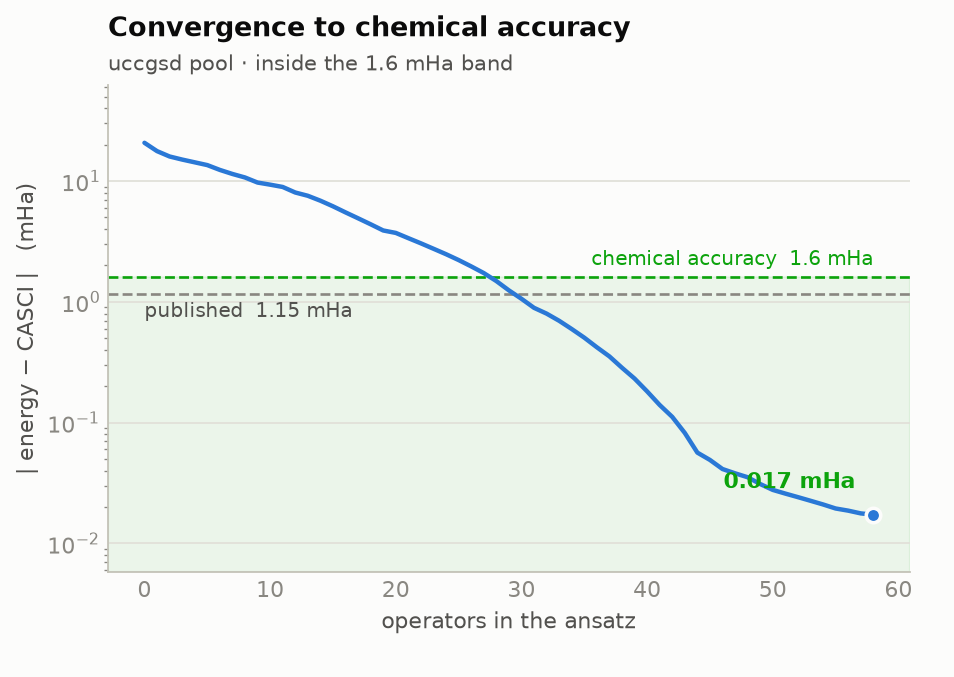
\includegraphics[width=0.66\textwidth]{figures/a-uccgsd-error.png}
\caption{ADAPT convergence with the \code{uccgsd} pool: error against CASCI on a
logarithmic axis, with the $1.6\mHa$ pass mark and the published $1.15\mHa$
statevector result drawn in. The trajectory crosses chemical accuracy well
before it stops.}
\label{fig:uccgsderr}
\end{figure}

\begin{figure}[htbp]
\centering
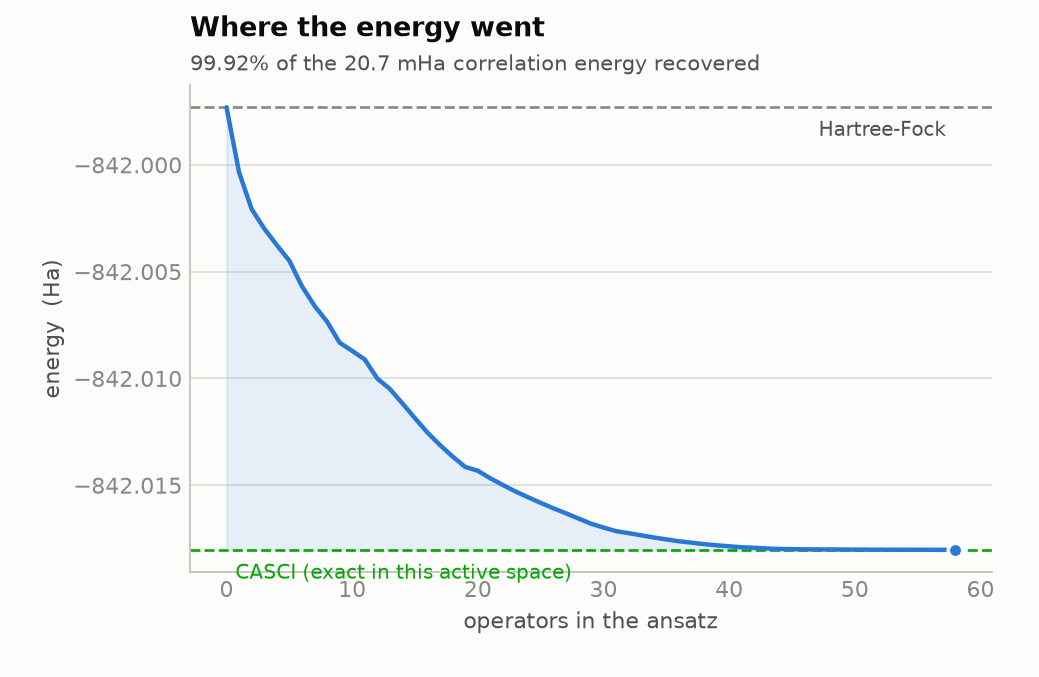
\includegraphics[width=0.66\textwidth]{figures/a-uccgsd-energy.png}
\caption{The same trajectory in absolute hartree, between the Hartree--Fock and
CASCI lines, so the recovered correlation is a visible distance rather than a
number to be trusted.}
\label{fig:uccgsdenergy}
\end{figure}

\begin{figure}[htbp]
\centering
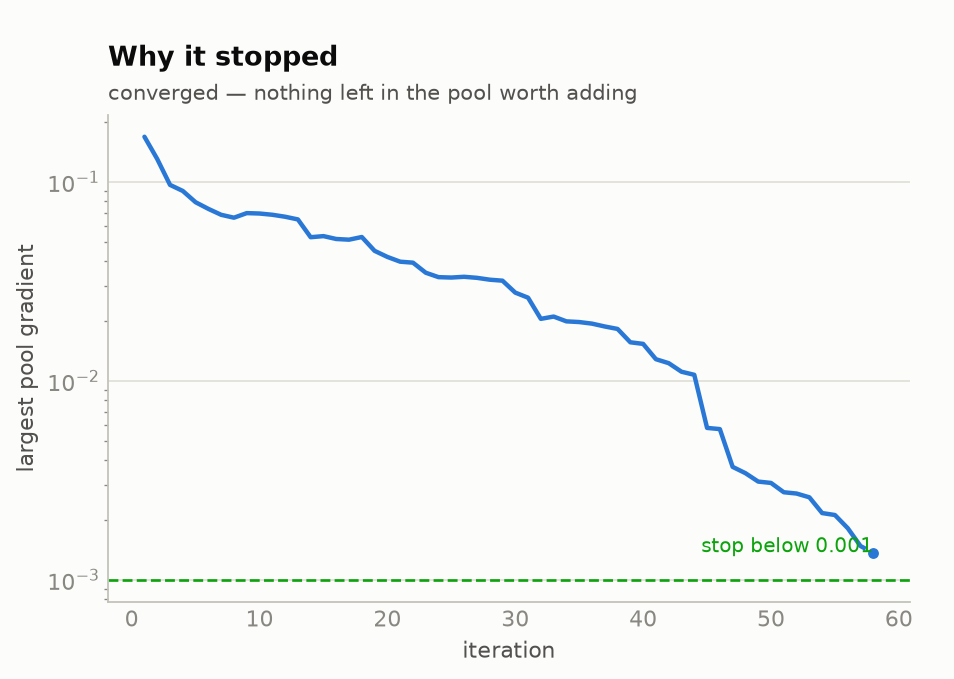
\includegraphics[width=0.66\textwidth]{figures/a-uccgsd-gradient.png}
\caption{The largest remaining pool gradient by iteration --- the termination
criterion. This run reaches the threshold; Figure~\ref{fig:uccsdgrad} does not,
and the difference between those two figures is the subject of
\S\ref{sec:notacomparison}.}
\label{fig:uccgsdgrad}
\end{figure}

\begin{figure}[htbp]
\centering
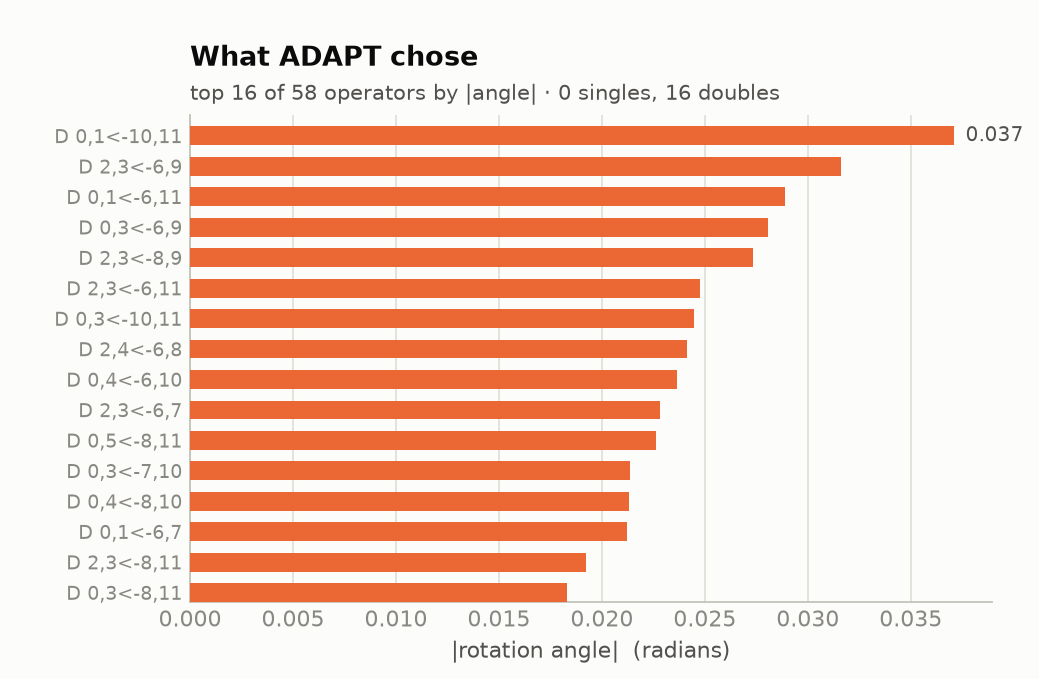
\includegraphics[width=0.72\textwidth]{figures/a-uccgsd-operators.png}
\caption{Selected operators by rotation angle, split into singles and doubles.
The correlation is carried by a small number of large-amplitude doubles.}
\label{fig:uccgsdops}
\end{figure}

\subsection{The \code{uccsd} run is not a pool comparison}
\label{sec:notacomparison}

\begin{figure}[htbp]
\centering
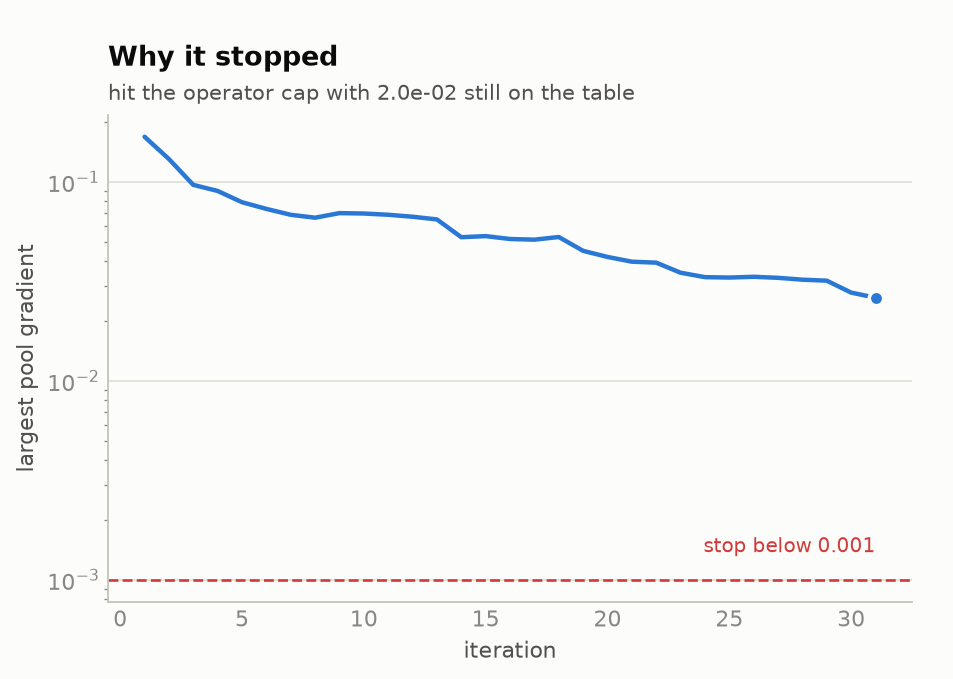
\includegraphics[width=0.66\textwidth]{figures/a-uccsd-gradient.png}
\caption{The \code{uccsd} run halting on its operator budget. The largest
remaining pool gradient at termination is $2.05\times10^{-2}$ --- twenty times
the stopping threshold of $10^{-3}$. The curve has not flattened.}
\label{fig:uccsdgrad}
\end{figure}

\begin{figure}[htbp]
\centering
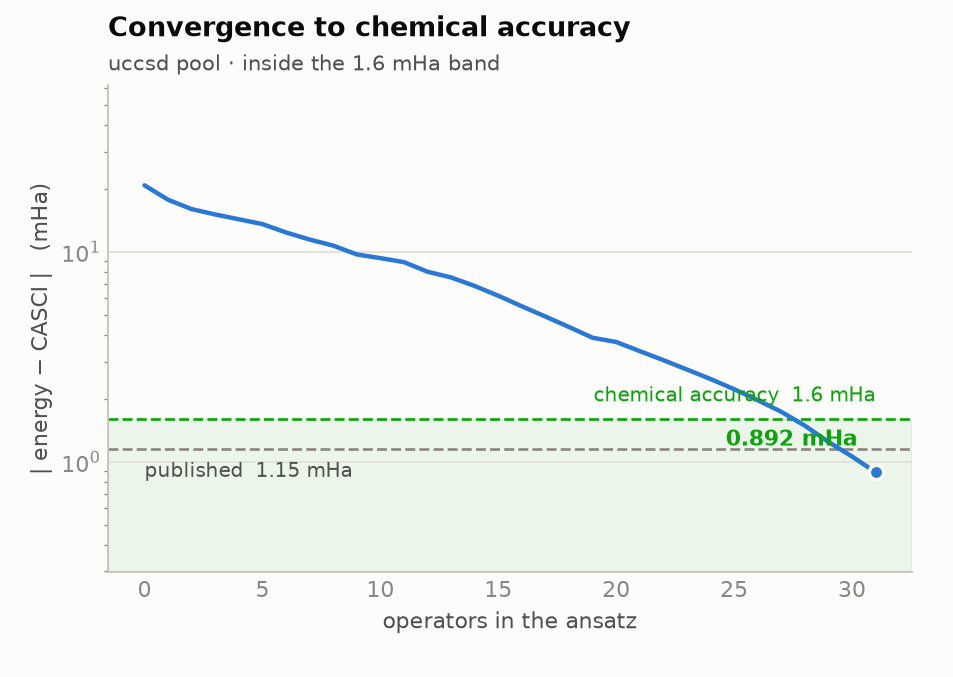
\includegraphics[width=0.66\textwidth]{figures/a-uccsd-error.png}
\caption{Error trajectory of the truncated run. It is still descending at the
point where it was stopped.}
\label{fig:uccsderr}
\end{figure}

\begin{unsupported}[The comparison that cannot be made]
Table~\ref{tab:runs} invites the reading that the generalized pool is a factor
of $52$ more accurate than the singles-and-doubles pool. That reading is not
supported. The \code{uccsd} run recorded
\code{stop\_reason: operator budget exhausted}, \code{converged: false}, and a
final pool gradient of $2.05\times10^{-2}$ against its threshold of $10^{-3}$.
It did not reach a stationary point. The two runs differ in \textbf{when they
were stopped}, not in what their pools can express, and separating those two
explanations requires re-running \code{uccsd} to its own gradient threshold with
the operator cap raised.
\end{unsupported}

This is a failure of experimental design, not of the algorithm, and it is
visible only because \code{stop\_reason} and \code{final\_pool\_gradient\_max}
are recorded in every result file. A result file carrying only the final energy
would have made the invalid comparison undetectable after the fact.

\subsection{The spin audit}
\label{sec:spin}

\begin{table}[htbp]
\centering
\caption{Symmetry diagnostics at the converged state. \emph{Priced} is the
contamination energy at $1\Ha$ per unit, against the $0.16\mHa$ budget of
\S\ref{sec:criteria}.}
\label{tab:spin}
\small
\begin{tabular}{lrrrl}
\toprule
Pool & $\Nop - 6$ & $\Ssq$ & Priced (mHa) & Verdict \\
\midrule
\code{uccgsd} & $0.0$ & $1.10\times10^{-6}$ & $0.0011$ & inside budget \\
\code{uccsd}  & $0.0$ & $2.76\times10^{-3}$ & $\mathbf{2.761}$ & \textbf{$17\times$ over} \\
\bottomrule
\end{tabular}
\end{table}

The \code{uccsd} run's energy is $0.892\mHa$ above CASCI. Against a threshold of
$1.6\mHa$, that reads as chemical accuracy, and would be reported as such by any
criterion that inspects the energy alone.

It is not. The converged state carries $\Ssq = 2.76\times10^{-3}$, which prices
at $2.761\mHa$ --- seventeen times the contamination budget, and more than three
times the error the run claims to have left. The state is not the closed-shell
singlet that the CASCI reference describes, so the comparison between the two
numbers is not between comparable objects.

\begin{result}[What one expectation value bought]
Measuring $\Ssq$ on the converged state costs a single expectation value against
a run of 9{,}188 matrix exponentials. It changed the verdict on that run from
\emph{chemical accuracy} to \emph{not usable}.
\end{result}

Note the relationship between this finding and \S\ref{sec:notacomparison}: they
are the same failure seen twice. The run did not converge, and a non-converged
ADAPT state is not obliged to be a spin eigenstate --- $S^2$ symmetry is
recovered at the variational minimum, and this run never reached one. The
remedy for both is identical: raise \code{--max-operators}, or lower
\code{--gradient-tolerance}, or use the seniority-zero \code{pair} pool whose
doubles commute with $S^2$ exactly.

\subsection{Circuit resources}

\begin{center}
\small
\begin{tabular}{lrr}
\toprule
& \code{uccgsd} & \code{uccsd} \\
\midrule
Two-qubit gates    & $4{,}241$ & $2{,}053$ \\
Single-qubit gates & $8{,}076$ & $4{,}243$ \\
Depth              & $6{,}977$ & $3{,}368$ \\
Optimisation level & $3$       & $3$ \\
Synthesis          & exact     & exact \\
\bottomrule
\end{tabular}
\end{center}

The circuit is constructed after the optimisation, transpiled at optimisation
level 3 for a gate count, and its energy re-evaluated. Both runs agree with
their algebraic energies below $10^{-9}\Ha$. These depths are far beyond current
hardware coherence for a 12-qubit device; the numbers are reported as a resource
estimate, not as a hardware proposal.

\subsection{Classical baselines in the identical active space}

\begin{table}[htbp]
\centering
\caption{Classical methods frozen to CAS(6e,6o), so the quantum error has a
scale. Errors against the CASCI reference.}
\label{tab:classical}
\small
\begin{tabular}{lrrr}
\toprule
Method & Energy (Ha) & Error (mHa) & Wall time (s) \\
\midrule
RHF        & $-841.9973061558$ & $20.736$ & $92.5$ (mean field) \\
MP2        & $-842.0102524898$ & $7.789$  & $5.7$ \\
CCSD       & $-842.0180213368$ & $0.021$  & $252.9$ \\
CCSD(T)    & $-842.0180339214$ & $\mathbf{0.008}$ & $502.1$ \\
\midrule
ADAPT \code{uccgsd} & $-842.0180246890$ & $0.017$ & $411.8$ \\
\bottomrule
\end{tabular}
\end{table}

\begin{caution}[What this benchmark can and cannot claim]
CCSD(T) reaches $0.008\mHa$ of the exact active-space answer in $502$ seconds;
ADAPT-VQE reaches $0.017\mHa$ in $412$ seconds. CAS(6e,6o) holds 400
determinants --- small enough that coupled cluster is already excellent and
exact diagonalisation is instant. \textbf{This is a verified reproduction, not a
demonstration of quantum advantage.} The classical ladder is computed and
reported so that the distinction is checkable rather than asserted.
\end{caution}

The CCSD note in the result file is worth repeating: CCSD is not exact here,
because a six-electron active space reaches hextuple excitations. The
perturbative triples correction is $-1.26\times10^{-5}\Ha$, an order of
magnitude smaller than the CCSD error itself, which is consistent with a
weakly correlated active space.

\subsection{Comparison with the published study}

\begin{center}
\small
\begin{tabular}{lr}
\toprule
Published (arXiv:2607.22468, Table 1) & \\
\midrule
CASCI energy                & $-841.953249\Ha$ \\
Statevector ADAPT-GQE       & $-841.952101\Ha$ \\
Statevector error           & $1.15\mHa$ \\
Hardware energy             & $-841.752841\Ha$ \\
Trained dataset accuracy    & $5$--$10\mHa$ \\
\bottomrule
\end{tabular}
\end{center}

\begin{caution}[Compare differences, not totals]
The published CASCI energy differs from the one here by $64.8\mHa$. That is a
conformer difference, not a disagreement: the geometry used here is a single
PubChem conformer and the published work uses a private conformer dataset. The
comparable quantity is $E_{\mathrm{CASCI}} - E_{\mathrm{HF}}$, i.e.\ the
correlation energy captured in the active space, and the error against each
study's own reference. On that basis $0.017\mHa$ here against $1.15\mHa$
published is a like-for-like statement; the total energies are not.
\end{caution}

\section{Discussion}

\subsection{A single failure mode, seen twice}

Both invalid comparisons in this study have the same shape: a quantity was
compared against a reference that described a different object. In
\S\ref{sec:notacomparison} the objects differed in operator budget; in
\S\ref{sec:spin} they differed in spin sector. In both cases the energies were
computed correctly, the optimiser reported success, and the resulting numbers
occupied a plausible range.

The instrumentation that caught them is three recorded quantities: the stop
reason, the largest remaining pool gradient, and $\Ssq$ at the optimum. None is
expensive. The first two are free --- the algorithm already computes them in
order to decide when to halt --- and the third is a single expectation value
against a run of tens of thousands of matrix exponentials. What they cost is
the discipline of writing them into the result file alongside the energy.

\subsection{Why the accuracy test is energetic}

Subtracting a penalty recovers $\langle \hat H \rangle$ exactly by linearity ---
but $\langle \hat H \rangle$ is a variational bound only \emph{within} the
six-electron sector, so a state that has leaked out of it can sit below CASCI
while meaning nothing. Demanding zero leakage would fail every physically
correct run of a hardware-efficient ansatz, which always leaks a little.

Pricing each broken symmetry at $1\Ha$ per unit and requiring the total below
$0.16\mHa$ --- one tenth of chemical accuracy --- makes the criterion decidable
and ensures that the contamination cannot be what produced the reported error.
The price is a convention, stated so the budget can be recomputed under a
different one.

\subsection{The $S^2$ penalty is off by default, and that is not a weakening}

Enabling the $\Ssq$ penalty adds several hundred Pauli terms to every energy
evaluation, to guard a secondary risk given a spin-free Hamiltonian, a
real-amplitude ansatz and a closed-shell start. It is therefore off. But $\Ssq$
is still \emph{measured} at the optimum and still priced into the same budget at
the full $1\Ha$ rate, so switching the penalty off cannot buy a weaker claim ---
as \S\ref{sec:spin} demonstrates, since that verdict was produced with the
penalty off.

\section{Claims not supported by these data}

\begin{enumerate}[leftmargin=1.4em,itemsep=0.3em]

\item \textbf{That \code{uccgsd} is a better pool than \code{uccsd}.} See
  \S\ref{sec:notacomparison}. Deciding it requires re-running \code{uccsd} to
  its own gradient threshold.

\item \textbf{That $0.892\mHa$ is what the \code{uccsd} pool can reach.} It is
  where a truncated run stopped, and the state there is spin contaminated.

\item \textbf{Any claim about imipramine as a molecule.} A single PubChem
  conformer, in vacuum, in 6-31G, with six electrons in six orbitals. The
  active-space correlation energy is $20.7\mHa$; the basis-set and
  active-space errors are not bounded by anything in this report and are
  certainly far larger.

\item \textbf{Any hardware claim.} The circuits of \S3.4 are resource estimates.
  Every energy in this report is a noiseless calculation, and the published
  hardware result for this system missed its own reference by $200\mHa$.

\item \textbf{Quantum advantage, in any form.} Table~\ref{tab:classical}
  forecloses it at this size.

\end{enumerate}

\section{Limitations}

\begin{enumerate}[leftmargin=1.4em,itemsep=0.2em]
\item One conformer, one geometry, one basis, one active space.
\item Two runs, one of which is invalid for two independent reasons. The
  \code{pair} pool was not run.
\item Seed 7; no statistics over initialisations. ADAPT is deterministic given
  the pool and the reference determinant --- the result files record
  \code{deterministic: true} --- so this is a smaller concern than for a
  randomly initialised VQE.
\item The results were produced on Colab with qiskit 1.0.2 and pyscf 2.14.0,
  which differs from the Windows environment the workflow also targets. Both are
  recorded in every result file.
\item The $1\Ha$ contamination price is a convention, not a derivation.
\end{enumerate}

\section{Conclusions}

\sloppy
\begin{enumerate}[leftmargin=1.4em,itemsep=0.25em]

\item ADAPT-VQE with a generalized pool reaches $0.0173\mHa$ of exact
  diagonalisation for imipramine in the CAS(6e,6o) active space, on twelve
  qubits, in $412$ seconds. It recovers $99.92\%$ of the correlation energy
  available there, its particle-number leakage is exactly zero, and no penalty
  term was used.

\item The emitted circuit --- 4{,}241 two-qubit gates, depth 6{,}977 ---
  reproduces that energy to $1.5\times10^{-12}\Ha$ under exact synthesis, so the
  result is a circuit result.

\item The second run does not support a pool comparison. It halted on an
  operator budget with a residual gradient twenty times its threshold, and its
  energy is separately invalidated by a spin contamination that prices at
  seventeen times the budget. Both were identified by quantities the algorithm
  already computes.

\item Classical CCSD(T) in the identical active space is more accurate and
  slower; exact diagonalisation of 400 determinants is instant. This is a
  verified reproduction with classical controls, and it is reported as such.

\end{enumerate}
\fussy

\appendix

\section{Provenance digests}

\begin{center}
\small
\begin{tabular}{ll}
\toprule
Quantity & Digest (first 16 hex) \\
\midrule
Molecular specification & \code{b85747c4a6092698} \\
Physics source          & \code{70982acc869f5f49} \\
ADAPT workflow          & \code{b31ea851aa093b65} \\
Hamiltonian cache       & \code{7a9d93ba991fe6c3} \\
Receipt penalty key     & \code{number=0,spin=0} \\
\bottomrule
\end{tabular}
\end{center}

Both runs carry identical cache, specification and physics digests, so they
solved the same operator.

\section{Complete settings}

\begin{center}
\small
\begin{tabular}{ll}
\toprule
Setting & Value \\
\midrule
Method                  & ADAPT-VQE \\
Backend                 & exact sparse statevector algebra (SciPy) \\
Gradient                & adjoint (exact) \\
Inner optimiser         & L-BFGS-B, tolerance $10^{-12}$, max 500 \\
Gradient tolerance      & $10^{-3}$ \\
Max operators           & $100$ (\code{uccgsd}), $31$ (\code{uccsd}) \\
Start                   & Hartree--Fock determinant, $\theta = 0$ \\
Number penalty          & $0.0\Ha$ \\
Spin penalty            & $0.0\Ha$ \\
Contamination price     & $1.0\Ha$ per unit \\
Contamination budget    & $1.6\times10^{-4}\Ha$ \\
Hamiltonian cutoff      & $10^{-6}\Ha$ \\
Circuit optimisation    & level 3 \\
Deterministic           & true \\
\bottomrule
\end{tabular}
\end{center}

The \code{uccsd} cap of 31 is the cause of \S\ref{sec:notacomparison}.

\section{Software environment}

Two stages, on two machines, and both are recorded in every result file.

The Hamiltonian and the classical ladder were built on Google Colab (Linux
6.6.122, Python 3.12.13, PySCF 2.14.0). That is the only stage requiring PySCF,
which publishes no Windows wheel.

Both ADAPT runs and the validation receipt reported here were produced on
Windows 11 / Python 3.13.7 with qiskit 2.3.1, qiskit-aer 0.17.2, OpenFermion
1.8.1, NumPy 2.4.3, SciPy 1.17.1. The same runs under qiskit 1.0.2 on Colab
reproduce the energies of Table~
ef{tab:runs} to the digits shown; only the
transpiled gate counts of Table~
ef{tab:exec} and the wall times differ, which
is what a transpiler version change should affect and all it should affect.

\section{Reproduction}

On a machine with PySCF (Linux, macOS, WSL or Colab):

\begin{verbatim}
python run.py prepare
python run.py classical
\end{verbatim}

Then anywhere:

\begin{verbatim}
python run.py validate --number-penalty 0 1 4
python run.py adapt --pool uccgsd
python run.py adapt --pool uccsd --max-operators 100   # the run that was
                                                       # truncated at 31
python run.py summary
python run.py plot
\end{verbatim}

\code{colab.ipynb} performs \code{prepare}, \code{validate} and \code{adapt} in
one free Colab session.

\section{Data inventory}

\begin{center}
\small
\begin{tabular}{ll}
\toprule
File & Contents \\
\midrule
\code{hamiltonian\_cas6e6o.json}           & the 12-qubit cache, 1{,}819 Pauli terms \\
\code{hamiltonian\_cas6e6o.validated.json} & its receipt, three penalty keys \\
\code{results/adapt\_uccgsd.json}          & the verified run \\
\code{results/adapt\_uccsd.json}           & the truncated, contaminated run \\
\code{results/classical.json}              & MP2, CCSD, CCSD(T) ladder \\
\code{results/adapt\_uccgsd.png}           & four-panel composite \\
\code{results/adapt\_uccsd.png}            & four-panel composite \\
\code{results/comparison.png}              & cross-run leaderboard \\
\bottomrule
\end{tabular}
\end{center}

Every quantity in this report is recomputable from those files. The composites
in \code{results/} are the sources of the individual panels reproduced as
Figures~\ref{fig:uccgsderr}--\ref{fig:uccsderr}.

\section*{References}
\small
\begin{enumerate}[leftmargin=1.4em,itemsep=0.1em]
\item R.\ Koziell-Pipe \emph{et al.}, arXiv:2607.22468 --- the Hamiltonian
  construction reproduced here, and the source of the published comparison.
\item H.\ R.\ Grimsley \emph{et al.}, \emph{An adaptive variational algorithm
  for exact molecular simulations on a quantum computer}, Nat.\ Commun.\
  \textbf{10}, 3007 (2019) --- ADAPT-VQE.
\item National Center for Biotechnology Information, PubChem CID 3696,
  imipramine --- the conformer used here.
\end{enumerate}

\end{document}
